\documentclass{standalone}
\usepackage{tikz}
\usetikzlibrary{decorations, decorations.text}
\usepackage{calc}
\usepackage{xcolor}
\usepackage{fontspec}

\setmainfont{Alegreya Sans}
\newcommand{\cevain}[1]{~{\fontspec{[ceva-c2.ttf]}#1} $\mid$ \emph{#1}}
\definecolor{eins}{HTML}{e7e7e8}   %% Ring 1 "core"     - weiß - Mittelpunkt, Ring um Mittelpunkt
\definecolor{zwei}{HTML}{ed1c24}   %% Ring 2 "com"      - rot -  "Fenster" innen
\definecolor{drei}{HTML}{fbad18}   %% Ring 3  "culture" - orange - fünf Module, quasi invertiert
\definecolor{vier}{HTML}{74c043}   %% Ring 4  "creactiv" - grün -  vier Module
\definecolor{fuenf}{HTML}{0089d0}  %% Ring 5 "cience"  - cyan (blau) - drei Module mit "Strich"
\definecolor{sechs}{HTML}{11357e}  %% Ring 6 "carbon" -  indigo - viele "Fenster" außen
\definecolor{sieben}{HTML}{000000} %% Ring 7 "clamp" -  schwarz, c-förmig
\definecolor{cbase}{HTML}{222222}  %% Körper der Raumstation    
\begin{document}
 
% \tikzset{
%   pics/carc/.style args={#1:#2:#3:#4}{
%     code={
%       \draw[postaction={decorate, decoration={text along path, raise=-2pt, text align={align=center}, text={\cevapic{#4}}, reverse path}}] (#1:#3) arc(#1:#2:#3);
%     }
%   }
% }%
    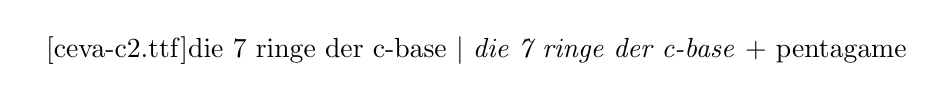
\begin{tikzpicture} 
        \node at (0,0) {\cevain{die 7 ringe der c-base} + pentagame};
    \end{tikzpicture}
\end{document}
